\section{Spændingsforsyning}
Spændingsforsyningen skal være i stand til at forsyne accelerometeret og EMG-forstækeren med en konstant spænding. Den anvendte spændingsforsyning er en færdigudviklet komponent, som består af to batterier på $1,5~V$, der sidder i en spændingsregulator. Batteriernes kobling danner et split supply, og derfor dannes der en jordforbindelse fra det ene batteris negative pol og den andens positive pol. De andre poler som ikke anvendes til jordforbindelse anvendes som systemets positive spændingsforsyning, {V}_{cc} og negative spændingsforsyning, {V}_{dd}.
Spændingsregulatoren sørger for give en jævnspænding på henholdsvis $3,4~V$ og $\pm 5,5~V$. Dette gøres ved, at spændingsregulatoren oplagre spænding fra de to tilkoblede batterier i spoler, når switchfunktionen lukkes. Switchfunktionen åbnes når spolerne er mættet og en spændingen ledes videre i kredsløbet via en diode. Denne switchfunktion åbner og lukker skiftevis i korttid, hvilket gør at der hele tiden ledes en konstant spænding til systemet. 
Konfigurationen af spændingsforsyningen fremgår af \autoref{fig:spaendingsforsyning}, hvor terminalerne for $\pm 5,5~V$ fremgår som rød(V+) og blå(V-) og sort(Gnd), mens der på den modsatte side fremgår terminalerne for $3,4~V$ som brun(Vcc) og sort(Gnd). 

\begin{figure}[H]
\centering
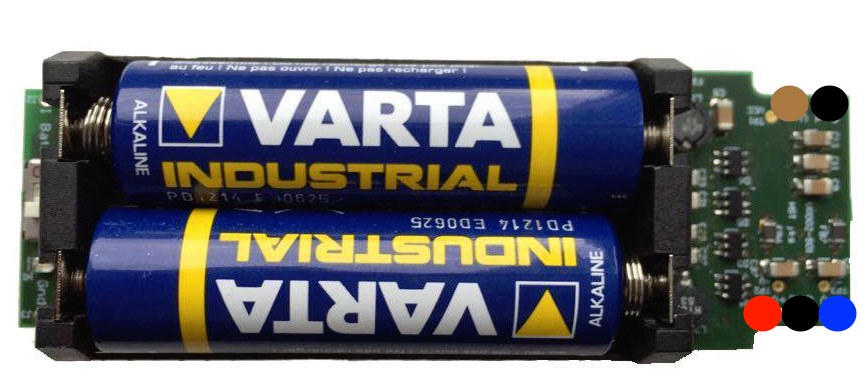
\includegraphics[width=0.6\textwidth]{figures/spaendingsforsyning.png}
\caption{Spændingsforsyningen der består af to $1,5~V$ batterier i et split supply}
\label{fig:spaendingsforsyning}
\end{figure}

\textbf{Krav:}
\begin{itemize} 
\item Skal kunne forsyne EMG forstærker
%\item Skal forsyne mikrokontrolleren
\item Accelerometeret skal forsynes af mikrokontrolleren
\item Skal være batteridrevet 
\end{itemize}
